\section{Introduction}
Language models (LMs), like other neural networks, often learn shortcuts from surface-level patterns in data. Early in training, LMs can behave like n-gram models, relying on local heuristics without capturing the deeper structure of language  \citep{Choshen2022-qj, Geirhos2020-ex, Saphra2018-xx}. However, LMs also exhibit breakthroughs in generalization, suddenly shifting from these simple heuristics to more sophisticated behaviors \citep{Choshen2022-qj, Chen2023-fi, McCoy2020-pj}. 
While previous works often attribute these advanced capabilities to model architecture and training objectives \citep{Ahuja2024-ul, McCoy2020-pj}, we investigate how \textit{data} characteristics influence which generalization rules models learn in ambiguous training settings. We also examine the training instabilities associated with generalization behaviors, and connect these dynamics to extreme variation across random seeds.


To understand when and why a model favors latent structures over surface-level heuristics, we use case studies in learning English grammar rules \cite{McCoyUnknown-uy}. 
Consider the example of a model inflecting a main verb to match the plurality of its subject. Figure \ref{fig:stability_demo} (\textit{bottom right}) shows an LM that uses a linear bigram model to capture the relationship between a subject noun and the main verb, applying a \textbf{linear rule}. This LM would fail to generalize when a \textit{distractor} noun, e.g., from a prepositional phrase, appears between subject and verb.
In contrast, Figure \ref{fig:stability_demo} (\textit{upper right}) shows a model that instead uses a latent tree structure to apply the correct syntactic rule (i.e., the \textbf{hierarchical rule}). This LM would generalize to any grammatical sentence. \citet{Murty2023-xp} showed that when trained long enough, LMs can switch from the surface-level heuristic to the hierarchical rule. They called this transition \textbf{structural grokking}, drawing a parallel to the famous grokking transition from memorization to generalization \citep{Power2022-hz}. 


\begin{figure}
    \centering
    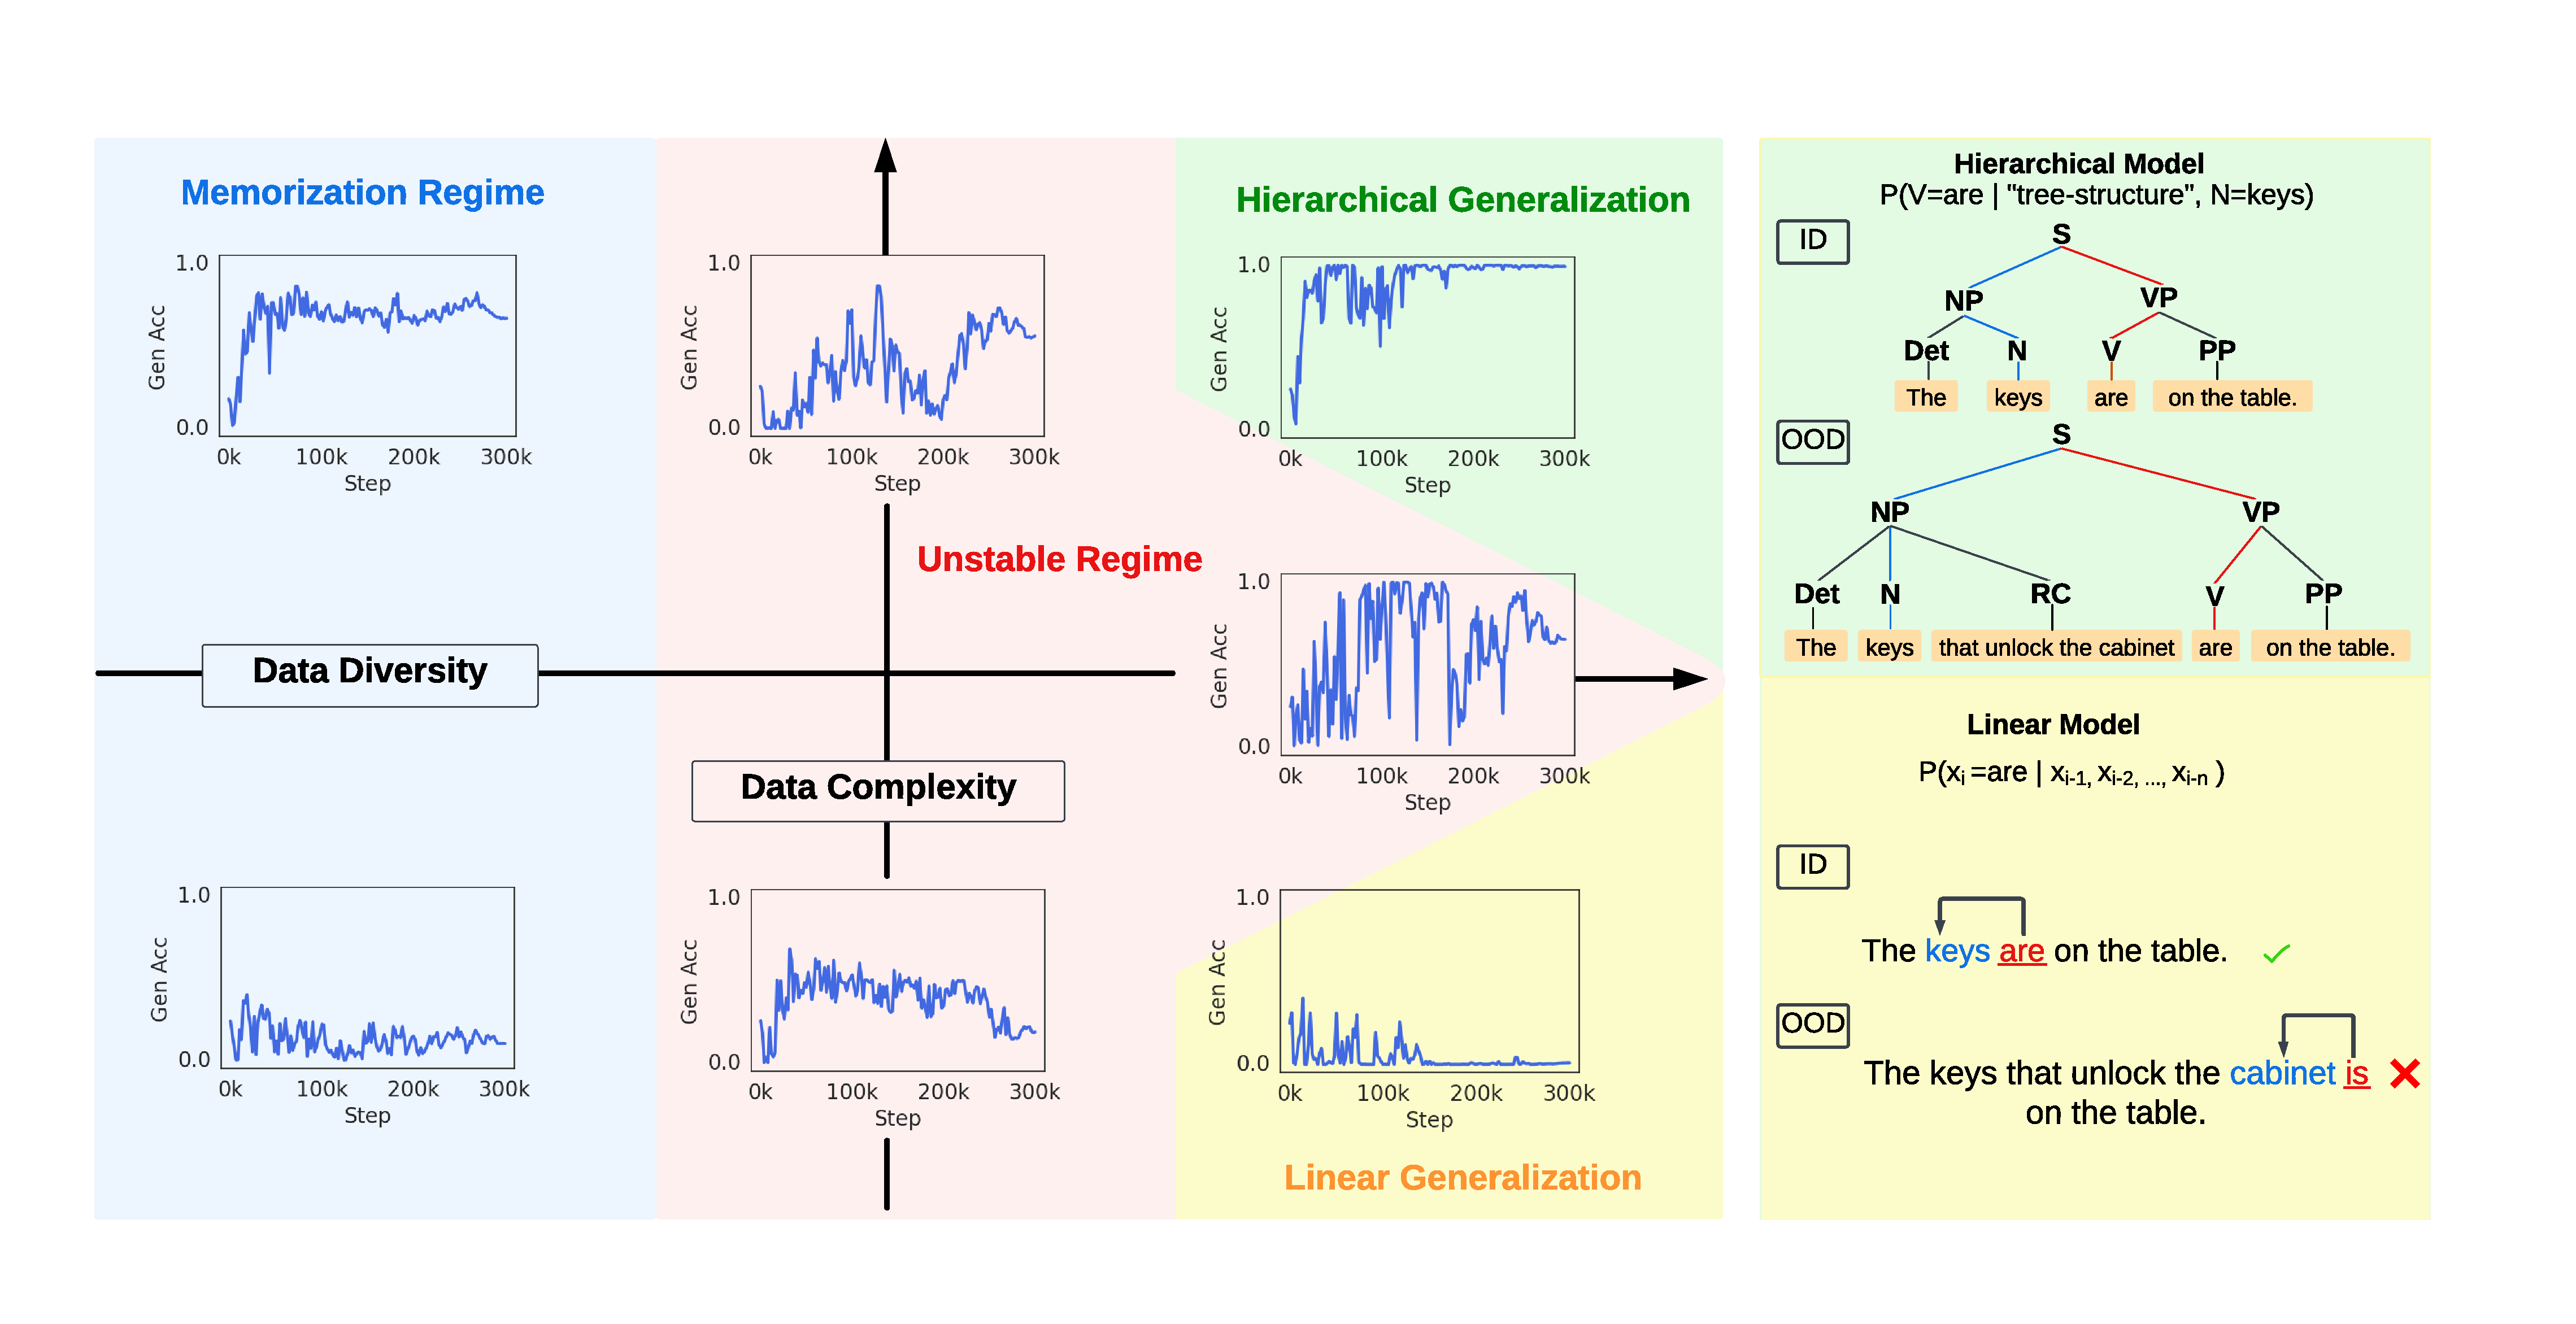
\includegraphics[width=1.0\textwidth]{figures/stability_demo.pdf}
    \caption{\textbf{Data plays a critical role in generalization behaviors and training stability.} 
    \textit{Left:} 
    Along the data diversity x-axis, low data diversity (as measured by variation in syntactic structure) leads the model to memorize unreliable sample-specific patterns, whereas high data diversity promotes commitment to a general rule. 
    Along the data complexity y-axis, high data complexity (as measured by the proportion of center-embedded sentences) induces the hierarchical rule, while simpler data (right-branching sentences) induces the surface-level linear rule. Mixing these data types results in unstable OOD training behaviors. 
    \textit{Upper Right:} A model that captures hierarchical structure of syntax can generalize grammatical rules OOD by correctly identifying the subject as the noun closest to the root on the syntax tree graph. 
    \textit{Lower Right:} A model that uses the linear rule will treat the most recent noun as the target verb's subject and thereby fail to generalize to unseen sentence compositions.
    } 
    \label{fig:stability_demo}
\end{figure}


Building on previous work \citep{McCoy2018-uv, McCoy2020-pj, Ahuja2024-ul, Murty2023-xp}, we investigate when a model learns the hierarchical rule, defaults to the surface-level linear rule, or fails to apply any systematic rule. We train models on ambiguous data, which is compatible with both the linear and hierarchical rules, and evaluate them on  out-of-distribution (OOD) data, which is compatible only with the hierarchical rule.
We first find that a preference for OOD hierarchical generalization is induced by training samples with center embeddings, where the subject is modified by an relative clause.  This result mirrors a celebrated claim from linguistics \citep{wexler1980formal} that center embeddings are responsible for human syntax acquisition. 


After identifying the data subset responsible for hierarchical generalization, we use grammar learning as a case study to understand the implications of rule competition on OOD behavior.
% in the consequences of competition between possible OOD behaviors. 
While the in-distribution behavior is always stable across time and consistent across random seeds, the model's OOD behavior is both \textbf{inconsistent} across seeds and \textbf{unstable} during training. 
Both the inconsistent training outcomes and the unstable training dynamics result from competition between different generalization rules. In particular, we show that only runs which systematically apply a general rule can exhibit stable OOD performance during training. 
To understand how the training data affects systematic rule learning, we precisely measure data complexity and diversity, relating these properties to distinct training dynamics regimes of memorization, generalization, and instability (Figure \ref{fig:stability_demo} \textit{left}). Specifically, we show that 
data diversity promotes a generalization rule over exact memorization, while data complexity determines which generalization rule is preferred. 


 
Taken together, our findings demonstrate that data composition plays a critical role in shaping a model's OOD generalization behavior. Our contributions are as follows:
\begin{itemize}[itemsep=2pt,labelindent=2pt,topsep=0pt,parsep=0pt,partopsep=1pt, align=left, leftmargin=*]
    \item Using case studies in grammar learning (Section \ref{sec:experiments}), we show that sentences with complex grammatical structure---specifically center embeddings---drive LMs to correctly favor hierarchical syntactic representations over surface-level n-gram heuristics (Section \ref{sec:data_complexity}). 
    \item We demonstrate that models stabilize in OOD performance only when they commit to either a surface-level heuristic or a hierarchical rule (Section \ref{sec:stability}). Furthermore, when the training data mixes complex and simple grammatical structures, the resulting rules are inconsistent across random seeds and many models fail to stabilize OOD behavior by the end of training. We posit that competition between different rules leads to both unstable training and inconsistent behavior across random seeds.
    \item We identify an exception to the relationship between stability and rule learning: Models trained on less diverse data stabilize in a memorization regime without learning either rule (Section \ref{sec:data_diversity}). In another example of how competition can destabilize training, we show that an intermediate level of diversity leads to greater instability than either low-diversity memorization or high-diversity generalization (Section \ref{sec:inverse}).
    \item This observation connects our study of transition between rules to the classic grokking scenario of transition from memorization to general rules. In both cases, the precarious competition which characterizes these transitions also leads to unstable dynamics and inconsistency across seeds.
\end{itemize}


